% Aalto Master's Thesis template
% Compatible with: UTF-8, pdflatex, biblatex, biber
%
% Compile using the following commands:
% $ pdflatex thesis.tex
% $ biber thesis
% $ pdflatex thesis.tex
% $ pdflatex thesis.tex
% $ pdflatex thesis.tex
%

\documentclass[12pt,a4paper,oneside,pdftex]{report}

\usepackage[utf8]{inputenc}
\usepackage[T1]{fontenc}
\usepackage[finnish,swedish,english]{babel}
%\usepackage[english]{babel}

\usepackage[section]{placeins}

\usepackage{mathtools}

% Font selection
%\usepackage{palatino}
%\usepackage[sc]{mathpazo}
\usepackage{kpfonts}
%\usepackage{tgpagella}
%\usepackage{garamond}
%\usepackage{lmodern}

% Verbatim provides a standard teletype environment that renderes
% the text exactly as written in the tex file. Useful for code
% snippets (although you can also use the listings package to get
% automatic code formatting).
\usepackage{verbatim}

% Longtable provides a tabular environment that can span multiple
% pages. This is used in the example abbreviations file.
\usepackage{longtable}

% The titlesec package can be used to alter the look of the titles
% of sections, chapters, and so on. This example uses the ``medium''
% package option which sets the titles to a medium size, making them
% a bit smaller than what is the default. You can fine-tune the
% title fonts and sizes by using the package options. See the package
% documentation.
%\usepackage[medium]{titlesec}
\usepackage[medium,raggedright]{titlesec}

\usepackage{subcaption}
\usepackage{graphicx}

\usepackage{tikz}
\usetikzlibrary{positioning}
\usetikzlibrary{calc}
\usetikzlibrary{arrows}
\usetikzlibrary{decorations.pathmorphing,decorations.markings}
\usetikzlibrary{shapes}
\usetikzlibrary{patterns}
\usetikzlibrary{automata}

\tikzset{initial text={}}
\tikzset{%
  zeroarrow/.style = {-stealth,dashed},
  onearrow/.style = {-stealth,solid},
  c/.style = {circle,draw,solid,minimum width=2em,
    minimum height=2em},
  r/.style = {rectangle,draw,solid,minimum width=2em,
    minimum height=2em}
}
\tikzset{
c/.style={
  circle,
  inner sep=0pt,
  text width=6mm,
  align=center,
  draw=black,
  fill=white
  }
}

\usepackage{amsthm}
\theoremstyle{definition}
\newtheorem{definition}{Definition}[section]

\usepackage{algorithm}
\usepackage[noend]{algpseudocode}
\renewcommand{\algorithmicrequire}[1]{\textbf{Input:} {#1}\\}
\renewcommand{\algorithmicensure}[1]{\textbf{Output:} {#1}}
\renewcommand{\algorithmicforall}{\textbf{for each}}
\newcommand{\Break}{\State\algorithmicbreak}

% Microtype for better typography
\usepackage[stretch=30,protrusion=true,final,expansion,tracking=true,kerning,spacing]{microtype}

% SI units. See table in 2lorem.tex for example
\usepackage{siunitx}
\sisetup{
    alsoload=binary
}

% Publication quality tables. See table in 2lorem.tex for example
\usepackage{booktabs}

% Use biber instead of bibtex as it supports UTF-8 among other things
\usepackage[backend=biber,
maxnames=5,
%style=numeric-verb,
style=alphabetic-verb, %numeric-comp %[1-3]
minalphanames=3,
maxalphanames=3,
sortcites=true,
%sorting=none
sorting=ydnt%Sort by year (descending), name, title 
%sorting=ynt %Sort by year, name, title. 
%sorting=nyt Sort by name, year, title. %see https://tex.stackexchange.com/a/51439
]{biblatex}
\renewcommand*{\labelalphaothers}{\textsuperscript{+}} %make the plus sign in bibliography references superscript


% Nicer looking caption for figures, tables, etc.
\usepackage[labelfont={bf},textfont={it},justification={raggedright},singlelinecheck={false}]{caption}

% Multiple figures inside one figure. See figure in 1lipsum.tex for example
%\usepackage{subfig}

% Inconsolata monospace font for verbatim environment
\usepackage{inconsolata}

% For rotating figures
\usepackage{rotating}

\usepackage{hyphenat} % for using \nohyphens

% Separate multiple citations with space instead of comma
% E.g. "[1] [2] [3]" instead of "[1], [2], [3]"
\renewcommand\multicitedelim{\space}

% Prevent orphan and widow rows
\widowpenalty=10000
\clubpenalty=10000

% Bibliography
\addbibresource{bib/ms-thesis.bib}

% The aalto-thesis package provides typesetting instructions for the
% standard master's thesis parts (abstracts, front page, and so on)
% Load this package second-to-last, just before the hyperref package.
% Options that you can use:
%   mydraft - renders the thesis in draft mode.
%             Do not use for the final version.
%   doublenumbering - [optional] number the first pages of the thesis
%                     with roman numerals (i, ii, iii, ...); and start
%                     arabic numbering (1, 2, 3, ...) only on the
%                     first page of the first chapter
%   twoinstructors  - changes the title of instructors to plural form
%   twosupervisors  - changes the title of supervisors to plural form
%\usepackage[mydraft,doublenumbering]{aalto-thesis}
\usepackage[doublenumbering]{lib/aalto-thesis}


% Hyperref
% ------------------------------------------------------------------
% Hyperref creates links from URLs, for references, and creates a
% TOC in the PDF file.
% This package must be the last one you include, because it has
% compatibility issues with many other packages and it fixes
% those issues when it is loaded.
\RequirePackage[pdftex]{hyperref}
% Setup hyperref so that links are clickable but do not look
% different
\hypersetup{colorlinks=false,raiselinks=false,breaklinks=true}
\hypersetup{pdfborder={0 0 0}}
\hypersetup{bookmarksnumbered=true}
% The following line suggests the PDF reader that it should show the
% first level of bookmarks opened in the hierarchical bookmark view.
\hypersetup{bookmarksopen=true,bookmarksopenlevel=1}
% Hyperref can also set up the PDF metadata fields. These are
% set a bit later on, after the thesis setup.


% Thesis setup
% ==================================================================
% Change these to fit your own thesis.
% \COMMAND always refers to the English version;
% \FCOMMAND refers to the Finnish version; and
% \SCOMMAND refers to the Swedish version.
% You may comment/remove those language variants that you do not use
% (but then you must not include the abstracts for that language)
% ------------------------------------------------------------------
% If you do not find the command for a text that is shown in the cover page or
% in the abstract texts, check the aalto-thesis.sty file and locate the text
% from there.
% All the texts are configured in language-specific blocks (lots of commands
% that look like this: \renewcommand{\ATCITY}{Espoo}.
% You can just fix the texts there. Just remember to check all the language
% variants you use (they are all there in the same place).
% ------------------------------------------------------------------
\newcommand{\TITLE}{\nohyphens{Automated Analysis of Weak Memory Models}} % TODO
\newcommand{\FTITLE}{?} % TODO
\newcommand{\SUBTITLE}{}
\newcommand{\FSUBTITLE}{}
\newcommand{\DATE}{?.?.2018} % TODO
\newcommand{\FDATE}{?.?.2018} % TODO

% Supervisors and instructors
% ------------------------------------------------------------------
% If you have two supervisors, write both names here, separate them with a
% double-backslash (see below for an example)
% Also remember to add the package option ``twosupervisors'' or
% ``twoinstructors'' to the aalto-thesis package so that the titles are in
% plural.
% Example of one supervisor:
\newcommand{\SUPERVISOR}{Assoc. Prof. Keijo Heljanko} % TODO
\newcommand{\FSUPERVISOR}{Assoc. Prof. Keijo Heljanko} % TODO
\newcommand{\SSUPERVISOR}{Assoc. Prof. Keijo Heljanko} % TODO

% If you have only one instructor, just write one name here
\newcommand{\INSTRUCTOR}{} % TODO
\newcommand{\FINSTRUCTOR}{} % TODO
\newcommand{\SINSTRUCTOR}{} % TODO
% If you have two instructors, separate them with \\ to create linefeeds
% \newcommand{\INSTRUCTOR}{Olli Ohjaaja M.Sc. (Tech.)\\
%  Elli Opas M.Sc. (Tech)}
%\newcommand{\FINSTRUCTOR}{Diplomi-insinööri Olli Ohjaaja\\
%  Diplomi-insinööri Elli Opas}
%\newcommand{\SINSTRUCTOR}{Diplomingenjör Olli Ohjaaja\\
%  Diplomingenjör Elli Opas}

% If you have two supervisors, it is common to write the schools
% of the supervisors in the cover page. If the following command is defined,
% then the supervisor names shown here are printed in the cover page. Otherwise,
% the supervisor names defined above are used.
%\newcommand{\COVERSUPERVISOR}{Professor Antti Ylä-Jääski, Aalto University\\
%  Professor Pekka Perustieteilijä, University of Helsinki}

% The same option is for the instructors, if you have multiple instructors.
% \newcommand{\COVERINSTRUCTOR}{Olli Ohjaaja M.Sc. (Tech.), Aalto University\\
%  Elli Opas M.Sc. (Tech), Aalto SCI}


% Other stuff
% ------------------------------------------------------------------
\newcommand{\PROFESSORSHIP}{} % TODO
\newcommand{\FPROFESSORSHIP}{?} % TODO check
% Professorship code is the same in all languages
\newcommand{\PROFCODE}{AS-116} % TODO check
\newcommand{\KEYWORDS}{Thesis template, master's thesis} % TODO
\newcommand{\FKEYWORDS}{Diplomityöpohja} % TODO
\newcommand{\LANGUAGE}{English} % TODO
\newcommand{\FLANGUAGE}{Englanti} % TODO

% Author is the same for all languages
\newcommand{\AUTHOR}{Artem YUSHKOVSKIY}

% Currently the English versions are used for the PDF file metadata
% Set the PDF title
\hypersetup{pdftitle={\TITLE\ \SUBTITLE}}
% Set the PDF author
\hypersetup{pdfauthor={\AUTHOR}}
% Set the PDF keywords
\hypersetup{pdfkeywords={\KEYWORDS}}
% Set the PDF subject
\hypersetup{pdfsubject={Master's Thesis}}


% Layout settings
% ------------------------------------------------------------------

% When you write in English, you should use the standard LaTeX
% paragraph formatting: paragraphs are indented, and there is no
% space between paragraphs.
% When writing in Finnish, we often use no indentation in the
% beginning of the paragraph, and there is some space between the
% paragraphs.

% If you write your thesis Finnish, uncomment these lines; if
% you write in English, leave these lines commented!
%\setlength{\parindent}{0pt}
%\setlength{\parskip}{1ex}

% Use this to control how much space there is between each line of text.
% 1 is normal (no extra space), 1.3 is about one-half more space, and
% 1.6 is about double line spacing.
\linespread{1.05}
% \linespread{1.3}

% Extra hyphenation settings
% ------------------------------------------------------------------
% You can list here all the files that are not hyphenated correctly.
% You can provide many \hyphenation commands and/or separate each word
% with a space inside a single command. Put hyphens in the places where
% a word can be hyphenated.
% Note that (by default) LaTeX will not hyphenate words that already
% have a hyphen in them (for example, if you write ``structure-modification
% operation'', the word structure-modification will never be hyphenated).
% You need a special package to hyphenate those words.
%\hyphenation{di-gi-taa-li-sta}


% Proper style for book binding, left margin bigger than right margin
% Uncomment to take into use
%\setlength{\parindent}{0pt}
%\setlength{\parskip}{2ex}
%\setlength{\textwidth}{140mm}
%\setlength{\oddsidemargin}{20mm}
%\setlength{\evensidemargin}{20mm}
%\setlength{\textheight}{240mm}
%\setlength{\voffset}{3mm}
%\setlength{\topmargin}{-11mm}


% The preamble ends here, and the document begins.
% Place all formatting commands and such before this line.
% ------------------------------------------------------------------
\begin{document}
% This command adds a PDF bookmark to the cover page. You may leave
% it out if you don't like it...
\pdfbookmark[0]{Cover}{bookmark.0.cover}
% This command is defined in aalto-thesis.sty. It controls the page
% numbering based on whether the doublenumbering option is specified
\startcoverpage

% Cover page
% ------------------------------------------------------------------
% Options: finnish, english, and swedish
% These control in which language the cover-page information is shown
  \coverpage{english}


% Abstracts
% ------------------------------------------------------------------
% Include an abstract in the language that the thesis is written in,
% and if your native language is Finnish or Swedish, one in that language.

% Abstract in English
% ------------------------------------------------------------------
\thesisabstract{english}{
In id fringilla velit. Maecenas sed ante sit amet nisi iaculis bibendum sed vel
elit. Quisque eleifend lacus nec ipsum lobortis ornare. Nam lectus diam,
facilisis eget porttitor ac, fringilla quis massa. Phasellus ac dolor sem, eget
varius lacus. Sed sit amet ipsum eget arcu tristique aliquam. Integer aliquam
velit sit amet odio tempus commodo. Quisque commodo lacus in leo sagittis vel
dignissim quam vestibulum. Cras fringilla velit et diam dictum faucibus.
Pellentesque at eros non mauris auctor euismod. Nullam convallis arcu vel lectus
sollicitudin rutrum. Praesent consequat, nisl at pretium posuere, neque arcu
dapibus lacus, ut sollicitudin elit velit ultricies libero. Vestibulum ante
ipsum primis in faucibus orci luctus et ultrices posuere cubilia Curae;

Nulla semper hendrerit molestie. Pellentesque blandit velit sit amet est
vestibulum faucibus. Nullam massa turpis, venenatis non mollis fringilla, mattis
et diam. Fusce molestie convallis elementum. Morbi nec lacus dapibus arcu mollis
gravida. Aliquam erat volutpat. Nam vitae magna nunc. Nunc ut ipsum at massa
porttitor vestibulum. Praesent diam lorem, ultrices nec vestibulum id, volutpat
nec lacus.
}

% Abstract in Finnish
% ------------------------------------------------------------------
\thesisabstract{finnish}{
Cras tincidunt bibendum erat, vel tincidunt diam porttitor aliquam. Donec sit
amet urna non felis placerat pharetra. Aenean ultrices facilisis nulla vitae
semper. Nullam non libero quis dui fermentum aliquam id vel eros. Praesent
elementum tortor quis sem congue iaculis sit amet eget nisl. Quisque erat
tortor, condimentum eu volutpat et, blandit et augue. Phasellus erat turpis,
pretium non feugiat id, posuere id velit. Vestibulum ut sapien felis, quis
convallis dui.

In elementum est eu nulla hendrerit feugiat. In sodales diam vel lacus cursus
tincidunt. Morbi nibh dui, imperdiet non vestibulum non, dignissim id risus. Sed
sollicitudin neque lectus, porttitor sollicitudin elit. Nulla facilisi. Nullam
in ante eu mi suscipit sollicitudin. Sed est velit, gravida facilisis varius
eget, tempus sed urna. Aliquam erat volutpat. Nam semper condimentum nisi.
Nullam scelerisque, metus nec sodales vulputate, purus augue venenatis urna, sit
amet mattis turpis nisl ac metus. Mauris nec odio ut neque condimentum vulputate
vel in turpis. Nulla facilisi. Nulla id tellus sapien, vitae blandit lorem.
}

% Acknowledgements
% ------------------------------------------------------------------
% Select the language you use in your acknowledgements
\selectlanguage{english}

% Uncomment this line if you wish acknoledgements to appear in the
% table of contents
%\addcontentsline{toc}{chapter}{Acknowledgements}

% The star means that the chapter isn't numbered and does not
% show up in the TOC
\chapter*{Acknowledgements} % TODO
In id fringilla velit. Maecenas sed ante sit amet nisi iaculis bibendum sed vel
elit. Quisque eleifend lacus nec ipsum lobortis ornare. Nam lectus diam,
facilisis eget porttitor ac, fringilla quis massa. Phasellus ac dolor sem, eget
varius lacus. Sed sit amet ipsum eget arcu tristique aliquam. Integer aliquam
velit sit amet odio tempus commodo. Quisque commodo lacus in leo sagittis vel
dignissim quam vestibulum. Cras fringilla velit et diam dictum faucibus.
Pellentesque at eros non mauris auctor euismod. Nullam convallis arcu vel lectus
sollicitudin rutrum. Praesent consequat, nisl at pretium posuere, neque arcu
dapibus lacus, ut sollicitudin elit velit ultricies libero. Vestibulum ante
ipsum primis in faucibus orci luctus et ultrices posuere cubilia Curae;

\vskip 10mm

\noindent Espoo, \DATE
\vskip 5mm
\noindent\AUTHOR

% Acronyms
% ------------------------------------------------------------------
% Use \cleardoublepage so that IF two-sided printing is used
% (which is not often for masters theses), then the pages will still
% start correctly on the right-hand side.
\cleardoublepage
% Example acronyms are placed in a separate file, abbreviations.tex
\addcontentsline{toc}{chapter}{Abbreviations}
\chapter*{Abbreviations}

% The longtable environment should break the table properly to multiple pages,
% if needed

\noindent
\begin{longtable}{@{}p{0.25\textwidth}p{0.7\textwidth}@{}}
AST & Abstract Syntax Tree \\
CPU & Central Processor Unit \\
DTA & Data-Transfer Object \\
OOP & Object-Oriented Programming \\
SMT & Satisfiability Modulo Theories \\
\textbf{TODO} & \textbf{MORE}
\end{longtable}



% Table of contents
% ------------------------------------------------------------------
\cleardoublepage
% This command adds a PDF bookmark that links to the contents.
% You can use \addcontentsline{} as well, but that also adds contents
% entry to the table of contents, which is kind of redundant.
% The text ``Contents'' is shown in the PDF bookmark.
\pdfbookmark[0]{Table of contents}{bookmark.0.contents}
\tableofcontents

% List of tables
% ------------------------------------------------------------------
% You only need a list of tables for your thesis if you have very
% many tables. If you do, uncomment the following two lines.
% \cleardoublepage
% \listoftables

% Table of figures
% ------------------------------------------------------------------
% You only need a list of figures for your thesis if you have very
% many figures. If you do, uncomment the following two lines.
% \cleardoublepage
% \listoffigures

% The following label is used for counting the prelude pages
\label{pages-prelude}
\cleardoublepage

%%%%%%%%%%%%%%%%% The main content starts here %%%%%%%%%%%%%%%%%%%%%
% ------------------------------------------------------------------
% This command is defined in aalto-thesis.sty. It controls the page
% numbering based on whether the doublenumbering option is specified
\startfirstchapter

% Add headings to pages (the chapter title is shown)
\pagestyle{headings}

% The contents of the thesis are separated to their own files.
% Edit the content in these files, rename them as necessary.
% ------------------------------------------------------------------
\chapter{Introduction}
\label{ch:introduction}

Most modern computer systems contain large parts that operate concurrently. Though system parallelising can improve its performance drastically, it opens numerous of problems connected to correctness, robustness and reliability, which makes the concurrent program design one of the most difficult problems of programming~\cite{mckenney2017parallel}.
% Most articles, presentations and books on concurrent programming start with words how hard it is.

Traditionally, studies related to concurrent programming concern on more fundamental theoretical questions of designing race-free and lock-free parallel algorithms, asynchronous data structures and synchronisation primitives of a programming language. Unfortunately,
when it comes to 
%in cases of 
the real-world concurrent programs, the algorithmic level of abstraction is not enough for guaranteeing their properties of correctness and reliability. The reasons of this fact lie in the code optimisations that both compiler and hardware perform in order to increase performance as much as possible. For instance, Figure~\ref{simple_wmm_x86} provides simple example of
unexpected state `\texttt{(0:EAX=0~/\textbackslash~1:EAX=0)}' reachable in x86 machines (such little examples that illustrate specific behaviours of a WMM are called \textit{litmus tests}).
%reordering of memory access instructions within single process allowed by the x86-TSO weak memory model, which potentially breaks the program logic. 
This behaviour is caused by write buffers used by all processors in x86 architecture. These buffers cache writes to shared variables, so that the writes to shared memory does not become visible by other processes immediately. In the example, the write `\texttt{MOV~[x],1}' performed in the process \texttt{P0} stores value~\texttt{1} into the shared variable~\texttt{[x]} in the write buffer of process~\texttt{P0}. Meanwhile, the write cache of the process \texttt{P1} may not have updated version of the variable~\texttt{[x]}, neither may have the main memory, so that the read `\texttt{MOV~EBX,[x]}' performed in the process~\texttt{P1} may read the initial value~\texttt{0}, even if this variable has been already updated in another thread. More presice description of x86-TSO memory model is given in Chapter~\ref{ch:wmm:x86}.

\begin{figure}
\small \ttfamily
\begin{tabular}{ |l|l| }
\hline
\multicolumn{2}{|l|}{ \{ x=0; y=0; \}} \tabularnewline \hline
P0 & P1 \\ \hline
MOV [x],1 & MOV [y],1 \\
MOV EAX,[y] & MOV EAX,[x] \\
\hline
%\multicolumn{2}{|l|}{locations [x;y;]} \tabularnewline
\multicolumn{2}{|l|}{exists (0:EAX=0~/\textbackslash~1:EAX=0)} \tabularnewline
\hline
\multicolumn{2}{|l|}{x86-TSO: allow} \tabularnewline
\hline

\end{tabular}
\caption{Litmus test of memory operations reordering allowed by the x86-TSO weak memory model}
\label{simple_wmm_x86}
\end{figure}

The first memory model for concurrent systems was formulated by Leslie Lamport back in 1979~\cite{lamport1979make}. This memory model, called the \textit{sequential consistency (SC) model}, allows only those executions (interleavings) that produce the same result as if the operations had been executed by single process. This means that the order of operations executed by a process is strictly defined by the program it executes. The SC model does requires the write to a shared variable performed in one process to become visible by all other processes not instantly, but simultaneously. This means each process communicates to the shared memory directly, without local buffering. Another important requirement of SC memory model is that it forbids memory operations reordering within single process (the order is strictly defined by the program).

The SC model is considered to be the strong memory model in the sence that it provides strong guarantees regarding the ordering and caused effect of memory operations. Different relaxations of this model lead to the class of \textit{weak memory models~(WMM)}.
%while preserving consistency
WMMs serve as set of guarantees made by designers of execution environment (hardware, programming language, compiler, database, operation system, etc.) to programmers on which behaviours of their concurrent code they may expect. 

Although weak memory studies is rather young research area, there exist frameworks and tools for exploring WMMs and examining simple programs with respect to the them. The state-of-the-art tool is \texttt{diy} (for \textit{do it yourself}), developed by the researchers from INRIA institute, France, and University of Cambridge, UK, and firstly released back in 2010. It is the sofware suite for designing and testing weak memory models, it consists of the litmus tests generators \texttt{diy7}, \texttt{diycross7} and \texttt{diyone7}, the litmus tests concrete executor \texttt{litmus7} that runs tests on a physical machine while collecting its behaviours, and the weak memory models simulator \texttt{herd7} that implements reachability analysis for capturing states allowed by the WMM. The latter tool uses systematic exhaustive search in a state space, which may be inefficient when analysing real-world programs, therefore more sophisticated search techniques should be applied for this problem. 

One possible approach is to use an efficient implementation of an SMT-solver (a SAT-solver extended by satisfiability modulo theories)~\cite{Porthos17}. % <-- TODO
This approach allows to capture symbolically the semantics of both the program and the weak memory model while encoding it into a single SMT-formula.
Most modern SMT-solvers are efficient enough to be able to operate the state space of size~??? [CITATION-?].

%In the work of Finnish and German researchers ... names ...
In the work~\cite{Porthos17}, the SMT-based approach was defined for analysing the portability of a program from one hardware architechture to another, which is defined as ``an execution that is consistent with the target but inconsistent with the source memory model". Although encoding the control-flow and the data-flow of a program into an SMT-formula seems to be a trivial problem of symbolic execution, encoding of the weak memory model is more tedious. The reason is that some relations of WMMs are defined as mutually-recursive and need to be linearised in order to be encoded into an equivalent logical formula.
%"a bounded model checking method that reduces the portability analysis problem to satisfiability modulo theorie" [Porthos17]
%"A portability bug is an execution that is consistent with the target but inconsistent with the source memory model. We capture this alternation with a single existential query. Consistency is specified in terms of acyclicity (and irreflexivity) of relations. Hence, an execution is inconsistent if a derived relation of the (source) memory model contains a cycle (or is not irreflexive)."

Current thesis aims to improve the proof-of-concept tool \texttt{PORTHOS} firstly introduced in April 2017 in the work~\cite{Porthos17} by extending the input language, which currently represents the minimum subset of C, and revising the general architecture of the tool in order to enhance performance, reliability and mantainability.

\section{Thesis structure}
\label{ch:introduction:structure}

The Chapter~\ref{ch:wmm} gives more detailed description of the weak memory models analysis and provides description of memory models for some common architectures (x86, ARM and POWER, Sparc, ???). Chapter~...
\chapter{Weak Memory Models}
\label{ch:wmm}

%"Semantics and verification under weak memory models have been the subject of study at least since 2007." [PORTHOS]
The \textit{weak memory model} is a set of predicative constraints on possible executions of a concurrent program. The study of formalisation the weak memory models for different architectures is being rapidly developed over last decade. Research of WMM aimes, firstly, to formalise the weak memory models and provide systematic, sound and complete formal approach of defining WMMs in order to be able to verify systems with respect to them.

%The generic framework of program analysis under weak memory models presented in~\ref{alglave2010shared} is discussed in Section~\ref{ch:wmm:event}.

Secondly, researchers work on extracting the formal hardware memory models from existing implementations of from their specifications, that are written in natural language and thus suffer from ambiguities and incompletenesses. Over last decade the memory models have been extracted for most mainstream multiprocessor architectures, such as x86-TSO (\textit{Total Store Order}) model for x86 architecture formalised in 2009~\cite{owens2009better}, SPARC-TSO for Sparc architecture~\cite{?!?!?!}, much more relaxed memory model ??? for Power and ARM architectures defined in ???~\cite{sarkar2011understanding}, Alpha (???). Moreover, in 2005 <who?Milner> started the work on developing the weak memory model for C++ language, which was introduced in C++11 (?) standard~\cite{???} (//todo: C11 MM ~\cite{batty2011mathematizing}). The memory model for Java that is based on the \textit{happens-before} principle was introduced in JVM??? in ??<year>. 

Thirdly, important research direction targets the problem of verifying (or at least finding bugs in) existing software systems with respect to weak memory models. In this <area> the notable works <are on> defining the Linux kernel memory model <that is being actively developing these days~\cite{kernel_wmm_1}>. Distributed databases <also need the wmm, see transaction consistency~\cite{bailis2013highly}>

%wmm as a formal way to define guaranties that a hw, programming language, execution environment provide for programmers.
%considering wmm as a set of allowed behaviours, the latter wmms are the supersets
%wmm allows and disallows optimisations: partial sync of memory buffers, out-of-order execution (reordering), <more> => more behaviours that are unallowed in SC.
%question possible to answer with wmm: which behaviours (in addition to SC) are allowed? which new states are allowed? Consequently, correctness, absence of data races, deadlocks or portability issues, etc.

%One important question that rises naturally when talking about weak memory models is whether a program is portable from one processor architecture to another. This can be solved ...<ref to PORTHOS>

% more examples of what wmms allow to do?

\section{The event-based program representation}
\label{ch:wmm:event}

%"The semantics of a program is a set of executions" https://johnwickerson.github.io/papers/memalloy.pdf


The classical approach to model the concurrent programs is to use the \textit{global time}, a single order of interleavings of all actions happened in different threads. However these models are easy to understand, it may be hard to consider \textit{all} possible states, number of which is exponentially large. Another way to do this is to to use non-deterministic computation-centric models defined in~\cite{fri97}, one of which represents the program as the graph of \textit{memory events}. The idea in this class of models is based on the fact that the behaviour of a concurrent system is defined only by the interleavings of shared-memory operations, while being independant from the order of local computation events. These models may be further restricted by constraints of a weak memory model, adding \textit{relations} to the memory events.
%Perhaps, the most convenient way to model the non-deterministic properties of concurrent programs is to use the program representation based on \textit{memory events}.
%In order to model the non-deterministic properties of concurrent programs 

The event-based program model represents the directed graph (\textit{event-graph}), where vertices represent \textit{events}, and edges represent \textit{relations} over the events. An event is something, that, after being executed, changes the state of an abstract machine executing the concurrent program. 
An \textit{execution} (trace, run) of a given program is an ordered set of events.
%associated with the instructions of the program
%the path in the event-graph. 
An execution is considered to be \textit{valid} if the memory events follow a single global timeline, i.e., can be embedded in a single partial order allowed by the memory model restrictions~\cite{alglave2010shared}. An execution to be checked on validity is called the \textit{candidate execution}.

Below we describe some basic types of events and relations.

\subsection{Events}
\label{ch:wmm:model:events}

A \textit{memory event} $e_m \in \mathbb{E}$ represents the fact of access to the memory. Since memory is the crucial low-level resource shared by multiple processes, most relations are defined over memory events. 
The processes can access a shared memory location (denoted by~$l_i$, for \textit{location}), or a local one (denoted by~$r_i$, for \textit{register}). A memory event is specified by its direction with respect to the shared variable, its location~$\texttt{loc}(e_m)$, its processor label~$\texttt{proc}(e_m)$, and a unique event label~$\texttt{id}(e_m)$~\cite{alglave2010shared}. 
%\texttt{load} for read the value of a shared-memory location, or \texttt{store} for write, or neither of them if both locations are local
The set of memory events $\mathbb{M}$ is devided into write events $\mathbb{W}$ (that write values to shared-memory locations) and read events $\mathbb{R}$ (that read values stored in shared-memory locations).
We add a restriction that each memory event uses at most one shared location, so that the write event $e_m = write(l_1, l_2)$ that writes value from shared location $l_2$ to the shared location $l_1$ is represented as two consequent events $e_m'~=~\texttt{load}(r_1 \leftarrow l_2); \ e_m''~=~\texttt{store}(l_1 \leftarrow r_1)$.

A \textit{computation event} $e_c \in \mathbb{C} \subseteq \mathbb{E}$, represents a low-level assembly computation operation performed solely on local-memory arguments. An example of computation event may be the event $e_c = r_3 \leftarrow add(r_1, r_2)$ that writes the sum of values stored in registers $r_1$ and $r_2$ to the register $r_3$. The \textit{control-flow} instructions (conditional and unconditional jumps) are encoded to the model directly, without additional events, as the $po$-relation (for \textit{program order}; see Chapter~\ref{ch:wmm:model:relations} for detailed definition of relations).

The third class of events is \textit{barrier events}, events caused by the synchronisation instructions (called \textit{fences}). Barrier events do not perform any computation or memory value transfer, instead, they add new relations to the model that restrict the set of allowed behaviours. Technically, a fence may either serve as a synchronisation barrier, or flush local memory caches, etc.


\subsection{Relations}
\label{ch:wmm:model:relations}

The basic relation in the event-based program model is the \texttt{po}-relation $\subset~\mathbb{E}~\times~\mathbb{E}$ (\textit{program-order}), which represents the total order of memory events \textit{within single process}, which never relates events from different processes. Thus, if a program specifies the memory instruction $i_2$ to follow immideately the memory instruction $i_2$, then there exist an edge $e_1 \xrightarrow{\texttt{po}} e_2$ in the event-graph where event $e_1$ is caused by the instruction $i_1$ and $e_2$ is caused by the instruction $i_2$. This relation encodes the control-flow of the program into the event-graph.
%Some new relations may be acquired : dp, po-loc

The data-flow of a program is encoded by the \textit{communication relations}: the \texttt{rf}-relation $\subset~\mathbb{W}~\times~\mathbb{R}$ (\textit{read-from} relation) that maps a write to a read reading its value, the \texttt{co}-relation $\subset~\mathbb{W}~\times~\mathbb{W}$ (\textit{coherence order}, sometimes called \texttt{ws}-relation for \textit{write serialisation}) defines the total order on writes to the same location across all processes, and the \texttt{fr}-relation $\subset~\mathbb{R}~\times~\mathbb{W}$ (\textit{from-read order}) that maps a read to possible writes preceding the current write event.
%TODO: perephrase last sentence! alglave thesis, p. 36

Figure~\ref{simple_wmm_x86_pic} illustrates the candidate execution for the Example~\ref{simple_wmm_x86}, that reaches the state \texttt{(0:EAX=0~/\textbackslash~1:EAX=0)} within x86-TSO memory model (the picture is generated by the \texttt{herd7} tool, version 7.47). 
%The event $b$:\texttt{(Ry=0)} reads value \texttt{0} at the shared location \texttt{y} from the initial write event $e$\texttt{(Wy=0)} (the red edge of \texttt{rf}-relation), consequently, 
%the event $d$:\texttt{(Rx=0)} reads value \texttt{0} at the shared location \texttt{x} from the initial write event $f$\texttt{(Wx=0)} (the red edge of \texttt{rf}-relation). 

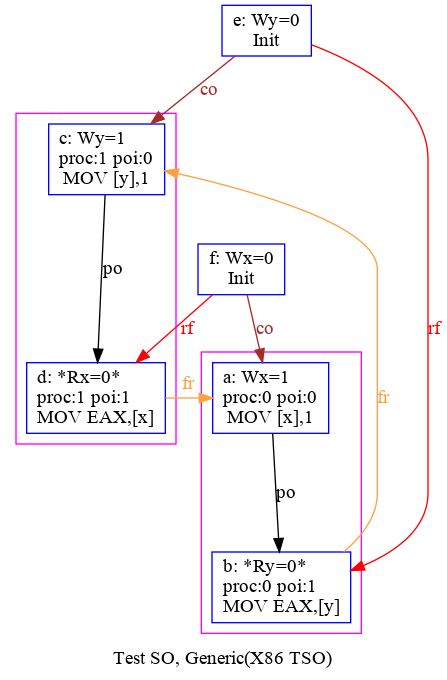
\includegraphics[width=0.4\textwidth]{img/my/simple_wmm_x86.png}
\label{simple_wmm_x86_pic}
% TODO: re-generate with new name, not 'SO'

\subsection{Executions}
\label{ch:wmm:model:executions}

The semantics of a concurrent program is represented by the set of allowed executions.
An execution is uniquely defined by the set $\mathbb{X}$ of events have been executed in each thread (the \textit{control-flow} of a program), and the relations $\mathtt{rf}$ and $\mathtt{co}$ (\textit{data-flow} of a program)~\ref{alglave2010shared}. As it was shown in~\ref{wickerson2017automatically}, it is enough for memory models to constrain the executions independently instead of constraining the program as a whole.

\section{The CAT language}

The Porthos tool uses the language \texttt{CAT}~\ref{alglave2016syntax} for defining weak memory models.

the event representation

\section{Some known WMM}

\subsection{x86-TSO}
\label{ch:wmm:x86}
// exmaple with reordering
// ex. with 
// Rev-29 Example 7-6. Stores Are Transitively Visible. %see http://www.cl.cam.ac.uk/~pes20/weakmemory/x86tso-paper.pdf

There is a barrier instruction \texttt{mfence} that may be used for flushing the buffers into the main memory.

briefly known hw memory models: X86-TSO, Alpha, POWER, -- ref to Jade;
language memory models: Java, C++;
library-level kernel memory model, ref to github with tests

Relationship between different models \url{http://wiki.expertiza.ncsu.edu/index.php/CSC/ECE_506_Spring_2013/10c_ks}

\chapter{Portability of Concurrent Software}
%\chapter{The Concurrent Software Portability Analysis as a Bounded Model Checking Problem}
\label{ch:port}

As it was discussed in Chapter~\ref{ch:intro}, the program may behave differently when compiled for different parallel hardware architectures. This can cause the portability bugs, the behaviour allowed under one architecture and forbidden under another. 
The concurrent software portability analysis may be stated as a Bounded Model Checking~(BMC) problem, which in turn can be reduced to the problem of satisfiability modulo theories (SMT)~\cite{Porthos17}.

\section{The model checking problem}
\label{ch:port:mc}

The classical model checking algorithms explore the state space of an abstract automata or a transition system in order to find states that violate the specification. The general schema of model checking is the following: firstly, the analysing system is being represented as a transition system, a finite directed graph with labeled nodes representing states of the system such that each state corresponds to the unique subset of atomic propositions, that characterise the behavioral properties of each state. 
Then, the system constraints are being defined in terms of a modal temporal logic with respect to the atomic propositions. Commonly, the Linear Temporal Logic~(LTL) or Computational Tree Logic~(CTL), along with their extensions, are used as a specification language due to the expressiveness and verifiability of their statements. 
In the described schema, the model checking problem is reducible to the reachability analysis, an iterative process of a systematic exhaustive search in the state space. This approach is called \textit{unbounded model checking (UMC)}.

However, all model checking techniques are exposed to the \textit{state explosion problem} as the size of the state space grows exponentially with respect to the number of state variables of the system. In case of modeling concurrent systems, this problem becomes much more considerable due to exponential number of possible interleavings of states.
Therefore, the research in model checking over past 40 years was aimed at tackling the state explosion problem, mostly by optimising search space, search strategy or basic data structures of existing algorithms.

%[-- TODO: REPHRASE
One of the first major optimising technique was symbolic model checking with binary decision diagrams (BDDs). In this approach, a set of states is represented by a BDD instead of by listing each state individually~\cite{clarke2012model}.
%--]
The BDD representation can be linear of size of variables it encodes if the ordering of variables is optimal, otherwise the size of BDD is exponential. The problem of finding such an optimal ordering is known as NP-complete problem, which makes this approach inapplicable in some cases.

The other idea is to use satisfiability solvers for symbolic exploration of state space~\cite{clarke2001bounded}. In this approach, the state space exploration consists of sequence of queries to the SAT-solver, represented as boolean formulas that encode the constraints of the model and the finite path to a state in the corresponding transition system.  
%This approach uses an iterative process of constructing queries to the SAT-solver as a boolean formula which encodes the constraints of the model and the finite path to a state in the corresponding transition system. 
Due to the SAT-solver. This technique is called \textit{bounded model checking (BMC)}, because the search process is being repeated up to user-defined bound $k$, which may result to incomplete analysis in general case. However, there exist numerous techniques for making BMC complete for finite-state systems~(e.g.,~\cite{shtrichman2000tuning}).

%For instance, the idea of grouping states with similar properties into equivalence classes lead to the concept of traces in concurrent systems proposed by A.~Mazurkiewicz in 1986~\cite{mazurkiewicz1986trace}. 

\section{The portability as a BMC problem}
\label{ch:port:enc}

A program $P$ is called portable from the source weak memory model $\mathcal{M_S}$ to the target memory model $\mathcal{M_T}$ if all executions consistent under $\mathcal{M_T}$ are consistent under $\mathcal{M_S}$~\cite{Porthos17}:

\begin{definition}[Portability]
Let $\mathcal{M_S}$, $\mathcal{M_T}$ be two weak memory models. A program $P$ is portable from $\mathcal{M_S}$ to $\mathcal{M_T}$ if 
$cons_{\mathcal{M_T}}(P) \subseteq cons{\mathcal{M_S}}(P)$
\end{definition}

Note, that the formulation of portability requirements against \textit{executions} is strong enough, as it implies the portability against \textit{states} (the \textit{state-portability})~\cite{Porthos17}.

It is possible to formulate this requirement as an SMT formula, so that the portability analysis problem becomes reduced to the BMC problem. The full SMT formula $\phi$ should contain encodings of control-flow ($\phi_{CF}$) and data-flow ($\phi_{DF}$) of the program, and assertions of both memory models: $\phi = \phi_{CF} \land \phi_{DF} \land \phi_{\mathcal{M_T}} \land \phi_{\lnot\mathcal{M_S}}$. The control-flow and data-flow encodings are standard for BMC~\cite{collavizza2006exploration}, they are described below. However, encoding of memory models requires additional techniques due to recursive definitions of relations, that were proposed in~\cite{Porthos17}.
%$The \phi_{\mathcal{M_T}}$ is an encoding of the derived relations and all assertions of
%, and φ ¬M S 

\subsection{Encoding of the control-flow constraints}
\label{ch:port:enc:cf}


\subsection{Encoding of the data-flow constraints}
\label{ch:port:enc:df}


\subsection{Encoding of the memory model constraints}
\label{ch:port:enc:wmm}


\chapter{Implementation}
\label{section:impl}

This chapter describes the architecture of the tool \texttt{mousquitaires} ...

language: java


\section{Program Requirements}
\label{section:impl:requirements}

- stability (tests)
- scalability (new features of language, new models, new tasks for a program -- e.g.!)
- transparency
- efficiency

\section{Program Components}
\label{section:impl:comp}

Big view

\subsection{C11 to YTree parser}
\label{section:impl:comp:ytree}

- The language-dependent syntax tree:
        - for now it's the C subset language which I called 'Cmin'; as a base, I used the C11 grammar from ANTLR github repository, then I simplified it a lot, cutting off many unnecessary C syntax features and making it more convenient for parsing. When developing the Cmin language, I kept in mind C elements that are necessary for processing the linux kernel code, though for now not the whole grammar element described in file 'Cmin.g4' are being implemented;
        - later I am going to add the litmus grammar as well;
        - in future, it will be not a problem to add any new C-like language;

- The language-independent abstract syntax tree (aliased 'Ytree', where 'Y' resembles branching of the tree):
        - all tree nodes in my code are prefixed with 'Y', see tentative (yet almost complete) class hierarchy in picture 'YEntity.png';
        - this AST contains very basic language elements according to the C execution model (statements and expressions);
        - converting the language-dependent syntax tree to the language-independent syntax tree is performed by Visitor pattern (e.g., for Cmin->Ytree conversion is made by 'CminToYtreeConverterVisitor')
        - minor changes are performed by converting to ytree representation: desugaring the target code, etc.


\subsection{YTree to XGraph event converter}
\label{section:impl:comp:xgraph}

- Then, the AST is being interpreted and converted to event-based representation (aliased 'Xrepr' for eXecution representation):
        - more low-level code representation (or high-level assembly);
        - I try to keep this representation close to the one you described in your papers: basic load \& store events, branching events, fence events;
        - this representation is being implementing these days, I've just started doing it (see current class hierarchy in the picture 'XEntity.png');
        
- After we acquired the event-based representation, we can perform some modifications/simplifications/optimisations on it (separately, allowing user to manage them):
        - converting to SSA form as one of necessary steps before encoding;
        - (more? -- I'm not thinking about it yet);


\subsection{XGraph to ZFormula (SMT) encoder}
\label{section:impl:comp:zformula}

- Then, this modified event-representation is being encoded to SMT formula and sent to the solver.



\section{Optimisations}

... in each stage
\chapter{Evaluation}
\label{section:eval}

\section{Comparison with PORTHOS}

\subsection{Unique Features}
\subsection{Performance}




\section{Comparison with HERD}

\subsection{Unique Features}
\subsection{Performance}


\chapter{Summary}
\label{ch:summary}



% Fix numbering of bibliography section
\cleardoublepage
\phantomsection

\addcontentsline{toc}{chapter}{\bibname}
\printbibliography

% Appendices go here
% ------------------------------------------------------------------
% If you do not have appendices, comment out the following lines
\appendix
\chapter{Lorem ipsum}
\label{section:appendix1}

Cras pharetra bibendum felis nec fringilla. Curabitur accumsan iaculis justo,
eget imperdiet erat malesuada sed. Quisque lorem eros, feugiat sollicitudin
adipiscing at, rutrum quis elit. Nulla non nisl nunc. Fusce vitae tortor non
enim vestibulum suscipit in imperdiet elit. Curabitur sit amet leo purus, quis
ornare dui. Suspendisse vel arcu vel diam iaculis adipiscing a sit amet mauris.
Vestibulum augue magna, placerat vitae sagittis in, iaculis quis sem. Proin ut
arcu pulvinar orci blandit iaculis. Etiam mauris lacus, luctus a dictum vel,
rhoncus non dui. Mauris est urna, varius eget egestas a, adipiscing nec odio.
Aenean iaculis nisi sed quam pretium aliquet. Quisque et mi lacus, nec porta
ante. Nunc sed ante id diam hendrerit interdum in vitae eros. Ut odio ligula,
commodo id volutpat non, tristique at odio.



% End of document!
% ------------------------------------------------------------------
% The LastPage package automatically places a label on the last page.
% That works better than placing a label here manually, because the
% label might not go to the actual last page, if LaTeX needs to place
% floats (that is, figures, tables, and such) to the end of the
% document.
\end{document}

